\subsection{MPC}

MPC は、離散時間モデル、有限ホライズン評価関数、状態推定、入力制約、数値最適化を各サンプル時刻で結合する制御方式である。

\begin{figure}[tb]
\centering
\setlength{\unitlength}{0.75mm}
\begin{picture}(160,78)
  \small
  \thinlines
  \put(4,40){\makebox(0,0)[r]{参照 $r_k$}}
  \put(6,40){\vector(1,0){22}}
  \put(28,32){\framebox(32,16){\shortstack{最適化器\\QP/NLP}}}
  \put(60,40){\vector(1,0){18}}
  \put(69,44){\makebox(0,0)[b]{適用入力 $u_k$}}
  \put(78,32){\framebox(28,16){対象}}
  \put(106,40){\vector(1,0){22}}
  \put(132,40){\makebox(0,0)[l]{出力 $y_k$}}
  \put(120,40){\line(0,-1){24}}
  \put(120,16){\vector(-1,0){48}}
  \put(96,18){\makebox(0,0)[b]{測定値 $y_k$}}
  \put(40,8){\framebox(32,16){\shortstack{推定器\\状態 $\hat{x}_k$}}}
  \put(56,24){\vector(0,1){8}}
  \put(60,28){\makebox(0,0)[l]{$\hat{x}_k$}}
  \put(78,40){\line(0,-1){8}}
  \put(78,32){\vector(-2,-1){20}}
  \put(80,28){\makebox(0,0)[l]{実入力}}
  \put(30,60){\framebox(34,12){\shortstack{予測モデル\\$x^+=f(x,u)$}}}
  \put(47,60){\vector(0,-1){12}}
  \put(72,60){\framebox(30,12){\shortstack{制約\\$\mathcal{X},\mathcal{U}$}}}
  \put(72,60){\vector(-1,-1){12}}
\end{picture}
\caption{MPC の閉ループ構造。参照、推定状態、予測モデル、制約集合から最適化問題を作り、解かれた入力列の先頭だけを対象へ適用し、測定出力で次の時刻に解き直す。}
\label{fig:mpc-architecture}
\end{figure}

\wfig{mpc-architecture} は MPC の最初の視覚的整理であり、ロバスト MPC、チューブ MPC、NMPC の離散化、ソルバ失敗時の安全側入力、実時間スケジューリングまでを一枚で完了させる図ではない。ここで確認する範囲は、参照と推定状態から有限ホライズン問題を作り、制約を満たす入力列を計算し、先頭の入力だけを対象へ加えて測定値で再び問題を作り直す、という基本的な信号経路である。

離散時間線形系
\begin{equation}
  x_{k+1}=A_dx_k+B_du_k
\end{equation}
に対し、ホライズン $N$ の MPC は
\begin{align}
  \min_{x_i,u_i}\quad &
  \sum_{i=0}^{N-1}(x_i^\T Qx_i+u_i^\T Ru_i)+x_N^\T P_fx_N,\\
  \text{subject to}\quad &x_{i+1}=A_dx_i+B_du_i,\\
  &x_i\in\mathcal{X},\quad u_i\in\mathcal{U},\\
  &x_0=x_k
\end{align}
を解く。得られた入力列の最初の $u_0$ だけを実機へ加え、次のサンプルで状態を測り直して問題を解き直す。これを後退ホライズン制御という。

\begin{figure}[tb]
\centering
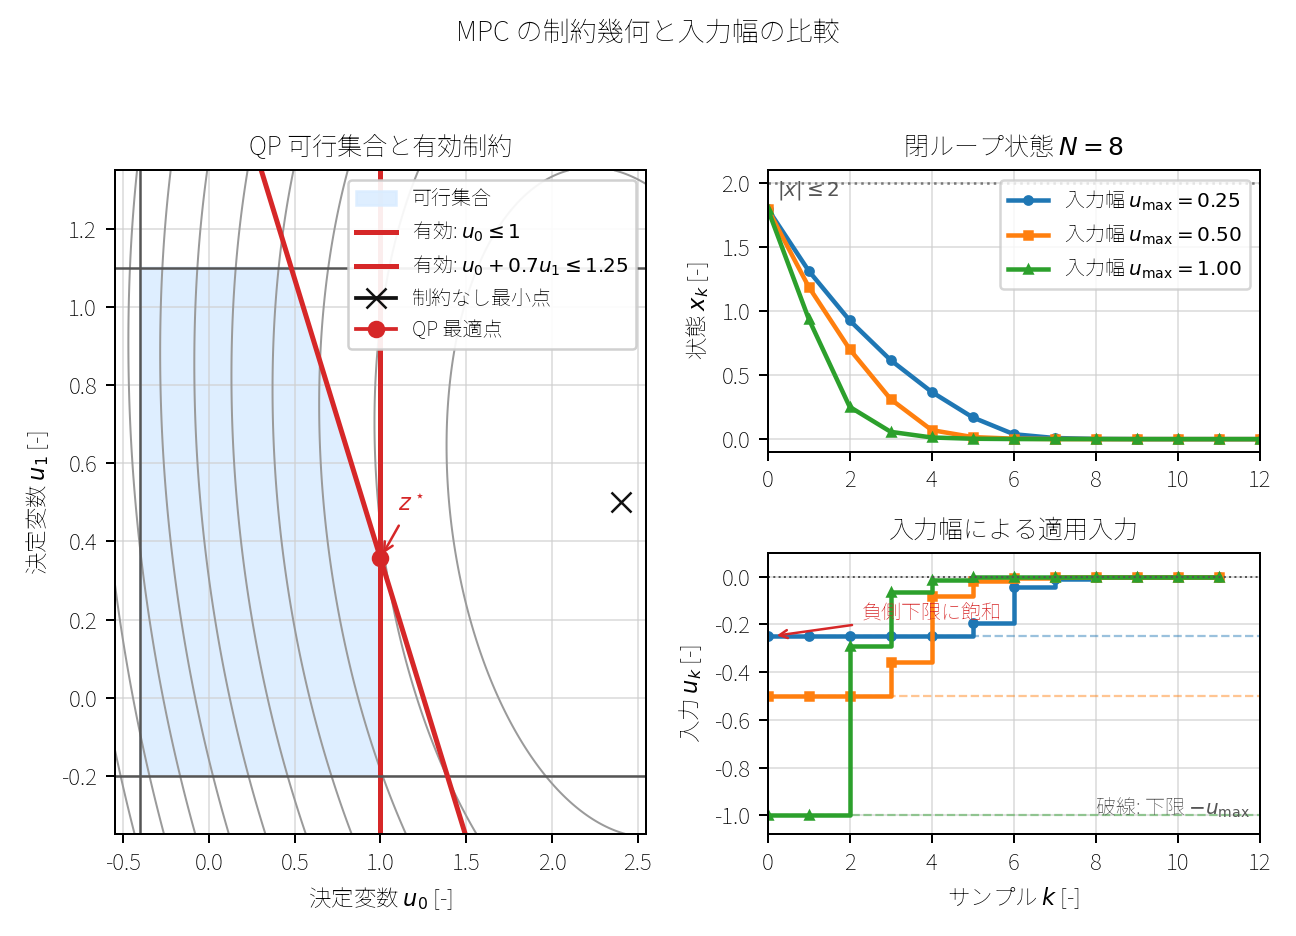
\includegraphics[width=0.94\linewidth,bb=0 0 1296 936]{figures/mpc_constraint_examples.png}
\caption{MPC と QP の制約を視覚化した例。左は決定変数 $z=(u_0,u_1)$ の可行集合、二次目的関数の等高線、制約なし最小点、制約付き最適点を示し、赤い境界が能動制約である。右は $x_{k+1}=0.8x_k+0.5u_k$、$N=8$、初期値 $x_0=1.8$ の閉ループで、入力上下限 $[-u_{\max},u_{\max}]$ を変えたときの状態と適用入力を比較している。入力幅が狭いほど負方向の下限 $-u_{\max}$ に張り付き、状態の減衰が遅くなる。}
\label{fig:mpc-constraint-examples}
\end{figure}

\wfig{mpc-constraint-examples} の左図では、制約なし最小点が可行集合の外にあるため、QP は可行多面体の境界上で最適点を選ぶ。赤い二本の境界は入力上限 $u_0\le1$ と、縮約後に $u_0+0.7u_1\le1.25$ の形で現れる結合線形制約を表し、両方が等号で満たされるので能動制約である。右図では同じ予測ホライズンでも、入力制約幅を狭くすると最初の数サンプルで $u_k$ が下限に張り付き、状態 $x_k$ の減少が遅くなる。したがって、MPC の調整では重み $Q,R$ だけでなく、制約幅、制約余裕、ホライズン長、終端条件が同じ閉ループ応答を決める。

\begin{practice}[MPC の制約余裕と能動制約の確認]
\wfig{mpc-constraint-examples} の左図で、制約なし最小点から制約付き最適点へ移るときに等号になる二つの不等式を特定し、KKT 乗数が正になり得る制約を答えよ。右図では $u_{\max}=0.25$ と $u_{\max}=1.00$ の場合について、$x_k<0.2$ になる最初のサンプル番号と、入力が制約に張り付いているサンプル数を比較し、入力制約幅が閉ループ応答へ与える影響を説明せよ。
\end{practice}

終端コスト $P_f$ に LQR のリカッチ解を使うと、ホライズンの先に続くコストを近似できる。終端制約
\begin{equation}
  x_N\in\mathcal{X}_f
\end{equation}
を置くと、制約条件のもとで実行可能性と安定性を解析できる。必要な仮定は、初期問題の実行可能性、終端集合の正不変性、終端コストの Lyapunov 不等式、実行可能な有限ホライズン問題に対して大域最適解を返す求解手順である。

\subsection{線形 MPC の終端条件と安定性}

以下では、添字 $d$ を省いて
\begin{equation}
  x_{k+1}=Ax_k+Bu_k
\end{equation}
と書く。状態と入力は平衡点まわりの偏差であり、原点 $(x,u)=(0,0)$ が制御したい点であるとする。制約集合 $\mathcal{X}$、$\mathcal{U}$ は原点を含む凸集合で、少なくとも MPC が使う範囲では閉じて有界であるとする。評価関数の一段コストを
\begin{equation}
  \ell(x,u)=x^\T Qx+u^\T Ru,
  \qquad Q\ge0,
  \qquad R>0
\end{equation}
とおく。有限ホライズン問題は
\begin{align}
  V_N(x_k)=\min_{x_i,u_i}\quad &
  \sum_{i=0}^{N-1}\ell(x_i,u_i)+V_f(x_N),\\
  \text{subject to}\quad &x_{i+1}=Ax_i+Bu_i,\\
  &x_i\in\mathcal{X},\quad u_i\in\mathcal{U},\\
  &x_N\in\mathcal{X}_f,\\
  &x_0=x_k
\end{align}
であり、終端コストはふつう
\begin{equation}
  V_f(x)=x^\T P_fx,
  \qquad P_f>0
\end{equation}
と選ぶ。

終端条件は、有限ホライズンの末端状態を、局所制御則により制約を保ったまま遷移できる集合へ制限する条件である。まず、原点近傍で制約を破らず安定化できる線形フィードバック
\begin{equation}
  u=K_fx
\end{equation}
を一つ固定し、閉ループ行列を
\begin{equation}
  A_f=A+BK_f
\end{equation}
と書く。終端集合 $\mathcal{X}_f$ は、少なくとも
\begin{align}
  \mathcal{X}_f&\subseteq\mathcal{X},\\
  K_fx&\in\mathcal{U}\qquad (x\in\mathcal{X}_f),\\
  A_fx&\in\mathcal{X}_f\qquad (x\in\mathcal{X}_f)
\end{align}
を満たすように選ぶ。三つ目の性質を正不変性という。つまり、終端集合へ入った状態は、終端制御則 $u=K_fx$ を使えば、次の時刻にも終端集合の中に残る。

終端コストは、終端集合の中で局所 Lyapunov 関数として働く必要がある。その条件は
\begin{equation}
  V_f(A_fx)-V_f(x)
  \le -\ell(x,K_fx)
  \qquad (x\in\mathcal{X}_f)
\end{equation}
である。左辺は終端制御則を一ステップ適用したときの終端コストの変化量であり、右辺はその一ステップのコストである。この不等式は、終端集合内で $K_f$ を適用した場合に、終端コストが一段コスト以上減少することを表す。

$K_f$ と $P_f$ の標準的な選び方は離散時間 LQR である。制約をいったん無視した無限ホライズン問題に対し、離散時間代数 Riccati 方程式
\begin{equation}
  P_f=A^\T P_fA
  -A^\T P_fB(R+B^\T P_fB)^{-1}B^\T P_fA+Q
\end{equation}
の安定化解 $P_f$ を取り、
\begin{equation}
  K_f=-(R+B^\T P_fB)^{-1}B^\T P_fA
\end{equation}
とする。このとき $A_f=A+BK_f$ は安定になり、
\begin{equation}
  A_f^\T P_fA_f-P_f=-(Q+K_f^\T RK_f)
\end{equation}
が成り立つ。両辺を $x^\T$ と $x$ で挟めば
\begin{align}
  V_f(A_fx)-V_f(x)
  &=x^\T(A_f^\T P_fA_f-P_f)x\\
  &=-x^\T(Q+K_f^\T RK_f)x\\
  &=-\ell(x,K_fx)
\end{align}
となり、終端 Lyapunov 条件が等号で満たされる。

終端集合は、制約を満たす正不変集合として構成する。多面体制約なら、まず
\begin{equation}
  \mathcal{S}_0=\{x\mid x\in\mathcal{X},\ K_fx\in\mathcal{U}\}
\end{equation}
を作り、
\begin{equation}
  \mathcal{S}_{j+1}=\{x\in\mathcal{S}_j\mid A_fx\in\mathcal{S}_j\}
\end{equation}
を繰り返す。ある段階で $\mathcal{S}_{j+1}=\mathcal{S}_j$ になれば、その集合は $A_f$ に対して正不変である。この集合を $\mathcal{X}_f$ として用いるか、その内側の楕円体または箱型集合を用いる。

\begin{theorem}[線形 MPC の再帰的実行可能性と安定性]
名目モデル $x_{k+1}=Ax_k+Bu_k$ が正確で、現在状態 $x_k$ が正確に利用でき、初期状態 $x_0$ で MPC 問題が実行可能であるとする。さらに、実行可能な有限ホライズン問題に対して求解手順が大域最適解を返し、終端集合 $\mathcal{X}_f$ が上の正不変性と制約条件を満たし、終端コスト $V_f$ が終端 Lyapunov 条件を満たすとする。このとき、閉ループの各時刻で MPC 問題は実行可能であり、最適値 $V_N(x_k)$ は一段コスト以上に減少する。特に $Q>0$ なら、再帰的実行可能な初期状態集合上で、原点は名目閉ループ系の漸近安定な平衡点である。
\end{theorem}

\begin{derivation}
時刻 $k$ の最適解を
\begin{equation}
  x^*_{0|k},x^*_{1|k},\ldots,x^*_{N|k},
  \qquad
  u^*_{0|k},u^*_{1|k},\ldots,u^*_{N-1|k}
\end{equation}
と書く。最初の入力 $u^*_{0|k}$ を実際に加えるので、名目モデルでは
\begin{equation}
  x_{k+1}=x^*_{1|k}
\end{equation}
である。次の時刻 $k+1$ では、前の最適列を一つ左へずらし、最後だけ終端制御則で補った入力列
\begin{align}
  \tilde{u}_{i|k+1}&=u^*_{i+1|k}\qquad (i=0,1,\ldots,N-2),\\
  \tilde{u}_{N-1|k+1}&=K_fx^*_{N|k}
\end{align}
を候補解として考える。この候補に対応する状態列は
\begin{align}
  \tilde{x}_{i|k+1}&=x^*_{i+1|k}\qquad (i=0,1,\ldots,N-1),\\
  \tilde{x}_{N|k+1}&=A_fx^*_{N|k}
\end{align}
である。前時刻の最適解が実行可能なので $x^*_{N|k}\in\mathcal{X}_f$ である。終端集合の正不変性より $K_fx^*_{N|k}\in\mathcal{U}$ かつ $A_fx^*_{N|k}\in\mathcal{X}_f$ が成り立つ。したがって、ずらした列は時刻 $k+1$ の実行可能解である。

次に最適値の減少を示す。時刻 $k+1$ の最適値は、任意の実行可能候補のコスト以下なので
\begin{align}
  V_N(x_{k+1})
  &\le
  \sum_{i=1}^{N-1}\ell(x^*_{i|k},u^*_{i|k})
  +\ell(x^*_{N|k},K_fx^*_{N|k})
  +V_f(A_fx^*_{N|k})\\
  &=V_N(x_k)-\ell(x^*_{0|k},u^*_{0|k})
  -V_f(x^*_{N|k})
  +\ell(x^*_{N|k},K_fx^*_{N|k})
  +V_f(A_fx^*_{N|k})\\
  &\le V_N(x_k)-\ell(x^*_{0|k},u^*_{0|k})
\end{align}
を得る。最後の不等式で終端 Lyapunov 条件を用いた。$Q>0$ かつ $R>0$ なら $\ell(x,u)$ は正定であるため、再帰的実行可能な状態集合上で $V_N$ は閉ループの Lyapunov 関数となる。$Q$ が半正定値の場合には、検出可能性に対応する追加条件が必要である。
\end{derivation}

一状態系の例を示す。平衡点まわりの温度偏差、または RC 回路の電圧偏差を表すモデルとして
\begin{equation}
  x_{k+1}=0.8x_k+0.5u_k
\end{equation}
とする。制約は
\begin{equation}
  \abs{x_k}\le2,
  \qquad
  \abs{u_k}\le1
\end{equation}
で、一段コストは
\begin{equation}
  \ell(x,u)=x^2+0.1u^2
\end{equation}
とする。終端制御則を $u=K_fx=-x$ と選べば、終端閉ループは
\begin{equation}
  x_{k+1}=(0.8+0.5(-1))x_k=0.3x_k
\end{equation}
である。終端コストを $V_f(x)=P_fx^2$ とし、終端 Lyapunov 条件を等号で満たすように選ぶと
\begin{align}
  V_f(0.3x)-V_f(x)&=-\{x^2+0.1(-x)^2\},\\
  (0.3)^2P_fx^2-P_fx^2&=-1.1x^2,\\
  P_f&=\frac{1.1}{1-(0.3)^2}\simeq1.209
\end{align}
となる。終端集合を
\begin{equation}
  \mathcal{X}_f=\{x\mid \abs{x}\le1\}
\end{equation}
とすれば、$x\in\mathcal{X}_f$ で $\abs{K_fx}=\abs{x}\le1$ だから入力制約を満たし、さらに $\abs{0.3x}\le0.3\le1$ だから次状態も $\mathcal{X}_f$ に残る。終端状態まで到達した予測列は、その先を $u=-x$ でつなげる。次のサンプルでは古い予測列を一つ捨て、最後にこの局所制御を付ければ、再び制約を満たす候補列が得られる。

この例において、終端集合は最終状態の参照値ではなく、局所制御則 $u=K_fx$ に対して正不変な制約集合である。$N$ を長くすれば終端集合へ到達可能な初期状態は増えるが、最適化変数の数も増える。逆に $N$ が短すぎると、制約のために終端集合へ到達できず、MPC 問題が実行不可能になる。

ソフト制約は、制約違反量を最適化変数として導入し、実行不可能性を緩和する定式化である。たとえば状態制約 $H_xx_i\le h_x$ を
\begin{align}
  H_xx_i&\le h_x+s_i,\\
  s_i&\ge0
\end{align}
に置き換え、評価関数へ
\begin{equation}
  \rho^\T s_i+s_i^\T S s_i,
  \qquad \rho>0,
  \qquad S\ge0
\end{equation}
を加える。スラック変数 $s_i$ は制約違反量であり、大きな重みを置けば、違反はできるだけ小さく抑えられる。しかし、ソフト制約は制約を守ったことの証明ではない。安全上越えてはならない状態制約や、物理的に出せない入力制約は原則としてハード制約のまま残す。特に入力制約をソフトにして最適化問題の中で $\abs{u}>u_{max}$ を許しても、実機のアクチュエータはその入力を出せない。

終端制約をソフト制約にする場合、$x_N\in\mathcal{X}_f$ を仮定したシフト列の実行可能性証明はそのまま成立しない。名目安定性の証明を保つには、終端集合と入力制約をハード制約として残すか、スラックを含む拡張問題に対して別の Lyapunov 不等式とペナルティ減少条件を示す必要がある。モデル誤差や外乱がある場合には、ソフト制約だけでは再帰的実行可能性は保証されない。制約保証には、外乱集合を考慮して制約を縮小するロバスト MPC またはチューブ MPC が用いられる。
